%%%%%%%%%%%%%%%%%%%%%%%%%%%%%%%%%%%%%%%%%%%%%%%%%%%%%%%%%%%%
%%  This Beamer template was created by Cameron Bracken.
%%  Anyone can freely use or modify it for any purpose
%%  without attribution.
%%
%%  Last Modified: January 9, 2009
%%
%%  http://cameron.bracken.bz/beamer-template

\documentclass[xcolor=x11names,compress]{beamer}

%% General document %%%%%%%%%%%%%%%%%%%%%%%%%%%%%%%%%%
\usepackage{graphicx}
\usepackage{tikz}
\usepackage{german}
\usetikzlibrary{decorations.fractals}
%%%%%%%%%%%%%%%%%%%%%%%%%%%%%%%%%%%%%%%%%%%%%%%%%%%%%%
%\setbeameroption{show notes on second screen=left}

%% Beamer Layout %%%%%%%%%%%%%%%%%%%%%%%%%%%%%%%%%%
\useoutertheme[subsection=false,shadow]{miniframes}
\useinnertheme{default}
\setbeamertemplate{footline}{%
\begin{beamercolorbox}{section in head/foot}
    \color{gray}\vskip2pt~  \insertshorttitle\hfill\insertpagenumber{} %
    of \insertpresentationendpage{} ~\vskip2pt
\end{beamercolorbox}
}
\usefonttheme{serif}
\usepackage{palatino}

\setbeamerfont{title like}{shape=\scshape}
\setbeamerfont{frametitle}{shape=\scshape}

\setbeamercolor*{lower separation line head}{bg=DeepSkyBlue4} 
\setbeamercolor*{normal text}{fg=black,bg=white} 
\setbeamercolor*{alerted text}{fg=red} 
\setbeamercolor*{example text}{fg=black} 
\setbeamercolor*{structure}{fg=black} 
 
\setbeamercolor*{palette tertiary}{fg=black,bg=black!10} 
\setbeamercolor*{palette quaternary}{fg=black,bg=black!10} 

\renewcommand{\(}{\begin{columns}}
\renewcommand{\)}{\end{columns}}
\newcommand{\<}[1]{\begin{column}{#1}}
\renewcommand{\>}{\end{column}}
%%%%%%%%%%%%%%%%%%%%%%%%%%%%%%%%%%%%%%%%%%%%%%%%%%
\title[Secure Hash Algorithm]{Secure Hash Algorithm}



\begin{document}

%%%%%%%%%%%%%%%%%%%%%%%%%%%%%%%%%%%%%%%%%%%%%%%%%%%%%%
%%%%%%%%%%%%%%%%%%%%%%%%%%%%%%%%%%%%%%%%%%%%%%%%%%%%%%
\begin{frame}
\title{Secure Hash Algorithm}
%\subtitle{SUBTITLE}
\subtitle{SHA-256}
\author{
	Chi Trung Nguyen\\
	{\it T-Systems}\\
}
\date{
	\begin{tikzpicture}[decoration=Koch curve type 2] 
		\draw[DeepSkyBlue4] decorate{ decorate{ decorate{ (0,0) -- (3,0) }}}; 
	\end{tikzpicture}  
	\\
	\vspace{1cm}
	\today
}
\titlepage
\end{frame}

%%%%%%%%%%%%%%%%%%%%%%%%%%%%%%%%%%%%%%%%%%%%%%%%%%%%%%
%%%%%%%%%%%%%%%%%%%%%%%%%%%%%%%%%%%%%%%%%%%%%%%%%%%%%%
\begin{frame}{Inhalt}
%\tiny
\tableofcontents%[pausesections]
\end{frame}

%%%%%%%%%%%%%%%%%%%%%%%%%%%%%%%%%%%%%%%%%%%%%%%%%%%%%%
%%%%%%%%%%%%%%%%%%%%%%%%%%%%%%%%%%%%%%%%%%%%%%%%%%%%%%

\section{\scshape Einf"uhrung}
\subsection{Was ist ein Hash?}
\begin{frame}{Was ist ein Hash?}

\begin{itemize}
\item deutsch:  \glqq\textit{zerhacken}\grqq, \glqq \textit{verstreuen}\grqq
	\pause
\item Hashfunktion oder Streuwertfunktion erstellt aus beliebiger gro"ser Quellmenge eine immer gleich gro"se Zielmenge
\begin{itemize}
\item $ f(x) = f(x') $
	\pause
\end{itemize}
\item Item C
\end{itemize}
\end{frame}


%%%%%%%%%%%%%%%%%%%%%%%%%%%%%%%%%%%%%%%%%%%%%%%%%%%%%%
%%%%%%%%%%%%%%%%%%%%%%%%%%%%%%%%%%%%%%%%%%%%%%%%%%%%%%
\section{\scshape Geschichte}
\subsection{SHA-0}
\begin{frame}{SHA-0}
\begin{itemize}
\item Item A
	\pause
\item Item B

\begin{itemize}
\item Subitem 1
\item Subtem 2
\end{itemize}

\item Item C
\end{itemize}
\end{frame}

%%%%%%%%%%%%%%%%%%%%%%%%%%%%%%%%%%%%%%%%%%%%%%%%%%%%%%
%%%%%%%%%%%%%%%%%%%%%%%%%%%%%%%%%%%%%%%%%%%%%%%%%%%%%%
\subsection{SHA-1}
\begin{frame}{SHA-1}

\end{frame}


%%%%%%%%%%%%%%%%%%%%%%%%%%%%%%%%%%%%%%%%%%%%%%%%%%%%%%
%%%%%%%%%%%%%%%%%%%%%%%%%%%%%%%%%%%%%%%%%%%%%%%%%%%%%%
\subsection{SHA-2}
\begin{frame}{SHA-2}

\end{frame}

%%%%%%%%%%%%%%%%%%%%%%%%%%%%%%%%%%%%%%%%%%%%%%%%%%%%%%
%%%%%%%%%%%%%%%%%%%%%%%%%%%%%%%%%%%%%%%%%%%%%%%%%%%%%%
\subsection{eig}
\begin{frame}[shrink=35]{eig}
\begin{table}[c]
\caption{Secure Hash Algorithmus Eigenschaften}
\begin{tabular}[ht]{|c|c|c|c|c|}
  \hline
  Algorithmus & Message Size(bits) & Block Size(bits) & Word Size(bits) & Message Digest Size(bits)\\
  \hline\hline
  SHA-1   & $<2^{64}$  &  512 & 32 & 160\\
  SHA-224 & $<2^{64}$  &  512 & 32 & 224\\
  SHA-256 & $<2^{64}$  &  512 & 32 & 256\\
  SHA-384 & $<2^{128}$ & 1024 & 64 & 384\\  
  SHA-512 & $<2^{128}$ & 1024 & 64 & 512\\  
  \hline
\end{tabular}
\label{tab:meinetabelle}
\end{table}
\end{frame}


%%%%%%%%%%%%%%%%%%%%%%%%%%%%%%%%%%%%%%%%%%%%%%%%%%%%%%
%%%%%%%%%%%%%%%%%%%%%%%%%%%%%%%%%%%%%%%%%%%%%%%%%%%%%%
\section{\scshape Implementierung}
\subsection{Algorithmus}
\begin{frame}{Funktionen}
$ Ch(E,F,G) = (E\wedge F) \oplus (\neg E\wedge G)$
$ Ma(A,B,C) = (A\wedge B) \oplus (A\wedge C) \oplus (B\wedge C)$\\
$ \Sigma_0 = (A\ggg 2) \oplus (A\ggg 13) \oplus (A\ggg 22) $\\
$ \Sigma_1 = (A\ggg 6) \oplus (A\ggg 11) \oplus (A\ggg 25) $\\
\end{frame}


%%%%%%%%%%%%%%%%%%%%%%%%%%%%%%%%%%%%%%%%%%%%%%%%%%%%%%
%%%%%%%%%%%%%%%%%%%%%%%%%%%%%%%%%%%%%%%%%%%%%%%%%%%%%%
\begin{frame}{Darstellung des Algorithmus}
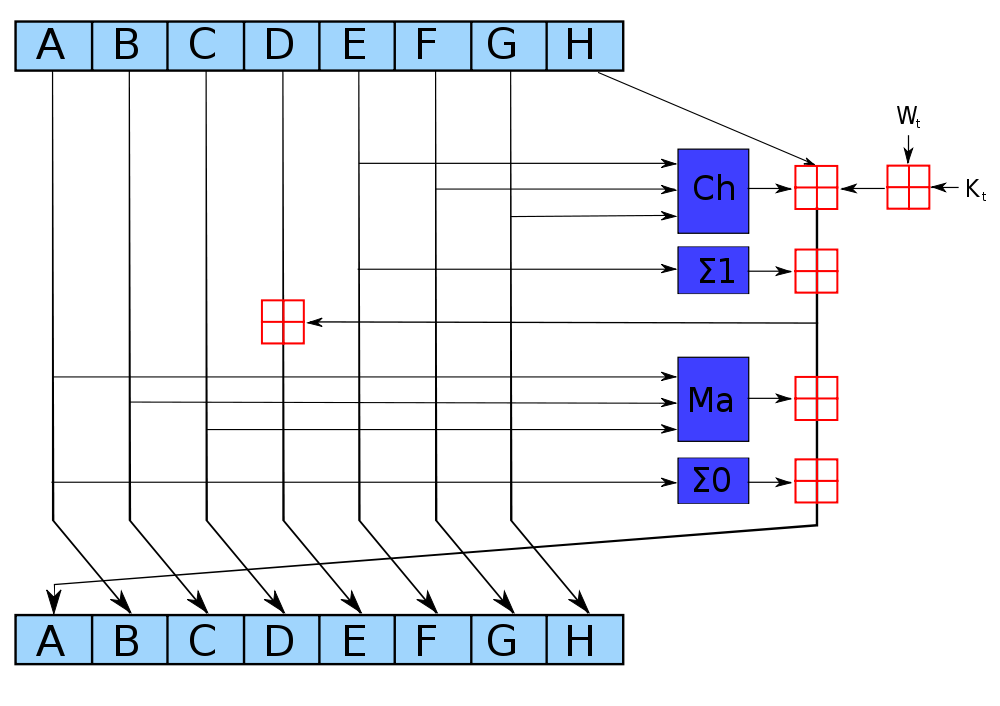
\includegraphics[scale=0.3]{sha256.png}\\
\end{frame}


%%%%%%%%%%%%%%%%%%%%%%%%%%%%%%%%%%%%%%%%%%%%%%%%%%%%%%
%%%%%%%%%%%%%%%%%%%%%%%%%%%%%%%%%%%%%%%%%%%%%%%%%%%%%%
\subsection{Pseudocode}
\begin{frame}{Pseudocode}

\end{frame}

%%%%%%%%%%%%%%%%%%%%%%%%%%%%%%%%%%%%%%%%%%%%%%%%%%%%%%
%%%%%%%%%%%%%%%%%%%%%%%%%%%%%%%%%%%%%%%%%%%%%%%%%%%%%%

\section{\scshape Anwendung}
\subsection{Verwendungszweck}
\begin{frame}{Verwendungszweck}

\end{frame}
%%%%%%%%%%%%%%%%%%%%%%%%%%%%%%%%%%%%%%%%%%%%%%%%%%%%%%
%%%%%%%%%%%%%%%%%%%%%%%%%%%%%%%%%%%%%%%%%%%%%%%%%%%%%%
\subsection{Sicherheitsl"ucken}
\begin{frame}{Sicherheitsl"ucken}

\end{frame}

%%%%%%%%%%%%%%%%%%%%%%%%%%%%%%%%%%%%%%%%%%%%%%%%%%%%%%
%%%%%%%%%%%%%%%%%%%%%%%%%%%%%%%%%%%%%%%%%%%%%%%%%%%%%%
\section{\scshape Ausblick}
\subsection{SHA-3}
\begin{frame}{SHA-3}

\end{frame}



\end{document}